\documentclass[a4paper,cs4size]{BHCexam}
%\documentclass[a4paper,cs4size,answers]{BHCexam}

\usepackage{multicol} % 分栏
\usepackage{hyperref}
\pagestyle{fancy}
\fancyfoot[C]{\kaishu \small 第 \thepage 页 共 \pageref{lastpage} 页}
%\fancyhead[L]{\includegraphics[width=2cm]{qrcode.png}}
\title{电路习题课2}
%\subtitle{数学文科试卷}
%\notice{满分150分, 120分钟完成, \\	允许使用计算器,答案一律写在答题纸上.}
%\author{Gavin Chen}
%\date{\today}

\begin{document}
\maketitle
\begin{groups}

    \group{}{例题}
    %\zihao{-4}
    \begin{questions}[]

        \question[5]三个阻值相等的电阻$R$和电阻$R_1$、$R_2$、$R_3$组成如图所示的电路,且$R_1=R_2=R_3$。若电阻$R_1$两端的电压为$20V$,
        电阻$R_3$两端的电压为$4V$,则电阻$R_2$两端的电压为(\quad\quad\quad)。
        \fourchoices{$6V$}
        {$8V$}
        {$10V$}
        {$12V$}
        \begin{figure}[htb]
            \flushright
            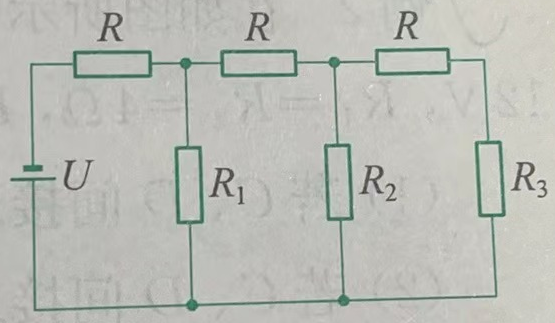
\includegraphics [scale=0.3,trim=0 0 0 0]{./image/physics_circuit2_1.png}
            % \caption{例1图}
            \label{fig:fig_circuit2_1}
        \end{figure}
        \vspace{2.5cm}

        \question[5]在如图所示的电路中,电流表的读数为$I$,若要使电流表的读数变为$4I$,则要(\quad\quad\quad)。
        \fourchoices{在电路中串联一个电阻$R_2$,且$R_2=3R_1$}
        {在电路中串联一个电阻$R_2$,且$R_2=\frac{R_1}{3}$}
        {在$R_1$两端并联一个电阻$R_2$,且$R_2=3R_1$}
        {在$R_1$两端并联一个电阻$R_2$,且$R_2=\frac{R_1}{3}$}
        \begin{figure}[htb]
            \flushright
            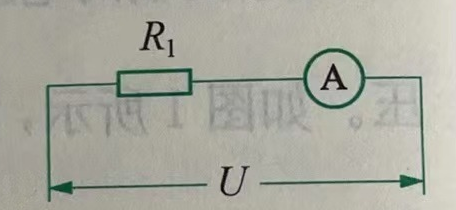
\includegraphics [scale=0.4,trim=0 0 0 0]{./image/physics_circuit2_2.png}
            % \caption{例2图}
            \label{fig:fig_circuit2_2}
        \end{figure}
        \vspace{2.5cm}

        \question[5]在如图所示的电路中,电阻$R_2<R_1$,若保持电路的总电流不变,那么为了使通过$R_1$的电流稍增大一点,可采用的措施是(\quad\quad\quad)。
        \fourchoices{与$R_2$并联一个比$R_2$小得多的电阻}
        {与$R_2$并联一个比$R_2$大得多的电阻}
        {与$R_2$串联一个比$R_2$小得多的电阻}
        {与$R_2$串联一个比$R_2$大得多的电阻}
        \begin{figure}[htb]
            \flushright
            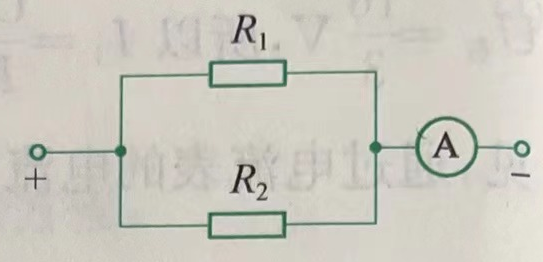
\includegraphics [scale=0.45,trim=0 0 0 0]{./image/physics_circuit2_3.png}
            % \caption{例3图}
            \label{fig:fig_circuit2_3}
        \end{figure}
        \vspace{2.5cm}


        \question[5]在如图所示的电路中,$R_1$的电阻值为$R$,$R_2$、$R_3$、$R_4$的电阻值都相等,电流表的电阻忽略不计,
        电路两端的电压恒定不变。当开关$S_1$、$S_2$同时合上或同时打开时,发现电流表的示数不变, 可以推知未知电阻$R_x$,的阻值为(\quad\quad\quad)。
        \fourchoices{$3R$}{$2R$}{$R$}{$\frac{1}{2}R$}
        \begin{figure}[htb]
            \flushright
            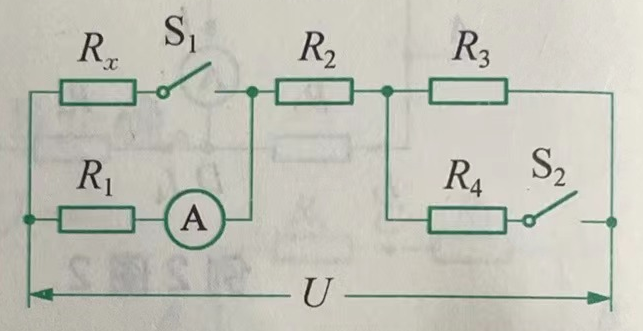
\includegraphics [scale=0.4,trim=0 0 0 0]{./image/physics_circuit2_4.png}
            % \caption{例4图}
            \label{fig:fig_circuit2_4}
        \end{figure}
        \vspace{2.5cm}

        \question[5]如图所示电路是由$12$个不同的电阻组成的,已知$R_1=12\Omega$,其余电阻阻值未知,测得$A$、$B$间的总电阻为$6\Omega$。
        今将$R_1$换成$6\Omega$的电阻,则$A$、$B$间的总电阻为(\quad\quad\quad)。
        \fourchoices{$6\Omega$}{$4\Omega$}{$3\Omega$}{$2\Omega$}
        \begin{figure}[htb]
            \flushright
            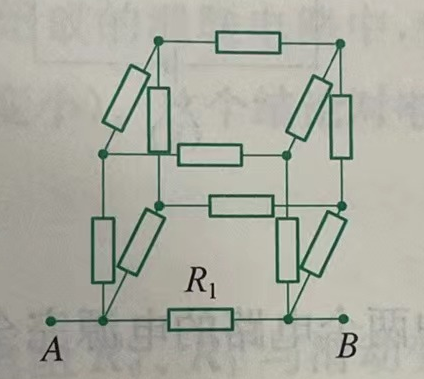
\includegraphics [scale=0.4,trim=0 0 0 0]{./image/physics_circuit2_5.png}
            % \caption{例5图}
            \label{fig:fig_circuit2_5}
        \end{figure}
        \vspace{2.5cm}

        \question[5]在如图所示的电路中,电源电压保持不变,开关$S$闭合前,电流表$A_1$、$A_2$ 的示数比为$5:3$,
        开关$S$闭合后,两电流表的示数比为$3:2$,则$R_1$、$R_3$的大小关系是(\quad\quad\quad)。
        \fourchoices{$R_1<R_3$}{$R_1>R_3$}{$R_1=R_3$}{无法确定}
        \begin{figure}[htb]
            \flushright
            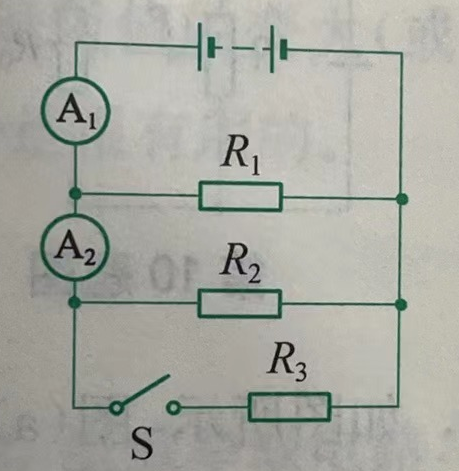
\includegraphics [scale=0.4,trim=0 0 0 0]{./image/physics_circuit2_6.png}
            % \caption{例6图}
            \label{fig:fig_circuit2_6}
        \end{figure}
        \vspace{2.5cm}

        \question[5]如图所示,滑动变阻器$R$的总电阻为$60\Omega$,定值电阻$R_0=60\Omega$,电源电压为$18V$。断开开关$S$,
        移动滑动片$P$使电压表的示数为$9V$,然后闭合开关$S$,则通过$R_0$的电流为(\quad\quad\quad)。
        \fourchoices{$0.12A$}{$0.15A$}{$0.24A$}{$0.45A$}
        \begin{figure}[htb]
            \flushright
            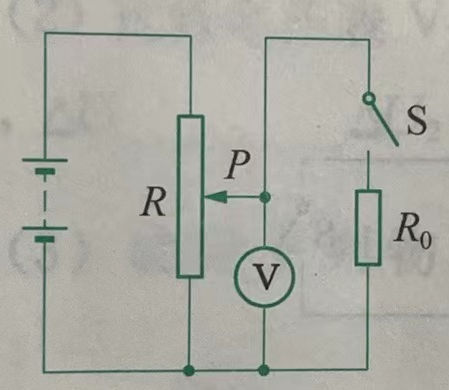
\includegraphics [scale=0.35,trim=0 0 0 0]{./image/physics_circuit2_7.png}
            % \caption{例7图}
            \label{fig:fig_circuit2_7}
        \end{figure}
        \vspace{2.5cm}

        \question[5]如图所示,图(a)、(b)中两个电路的电源完全相同,且$R_1=R_2=R_3\neq R_4$。
        则下列说法中正确的是()(\quad\quad\quad)。
        \fourchoices{电流表$A_1$没有示数,电流表$A_2$有示数}
        {电流表 $A_1$、$A_2$都有示数,且示数相同}
        {电流表$A_1$、$A_2$都有示数,且电流表$A_1$的示数较大}
        {电流表$A_1$、$A_2$都有示数,且电流表$A_2$的示数较大}
        \begin{figure}[htb]
            \flushright
            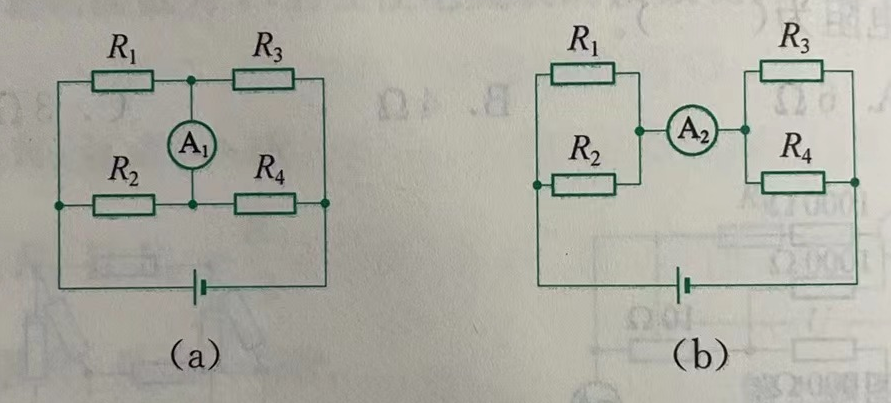
\includegraphics [scale=0.35,trim=0 0 0 0]{./image/physics_circuit2_8.png}
            % \caption{例8图}
            \label{fig:fig_circuit2_8}
        \end{figure}
        \vspace{2.5cm}



        \question[5]如图(a)所示,在一个电阻均匀的金属圆环上有$A$、$B$、$C$、$D$四点。其中$O$为圆心,
        $AB$、$CD$为圆环的两条互相垂直的直径。现把$A$、$B$两点接入电源电压保持不变的如图(b)所示的电路$M,N$ 两端时,
        发现电流表示数$I_0$,当换接$A$、$D$ 两点时,电流表的示数应为(\quad\quad\quad)。
        \fourchoices{$\frac{I_0}{4}$}{$\frac{3I_0}{4}$}{$I_0$}{$\frac{4I_0}{3}$}
        \begin{figure}[htb]
            \flushright
            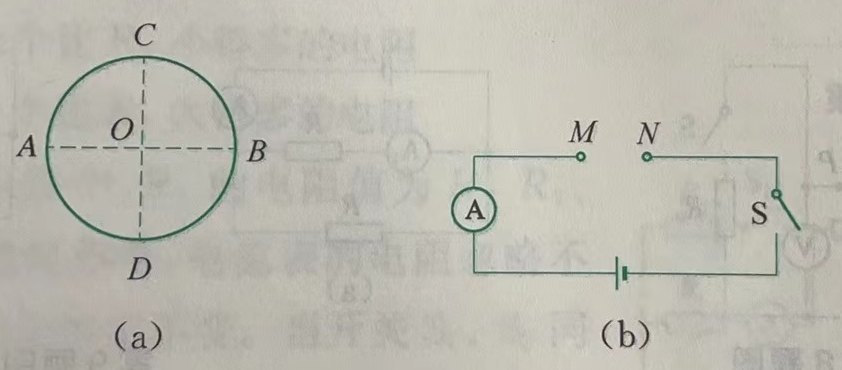
\includegraphics [scale=0.35,trim=0 0 0 0]{./image/physics_circuit2_9.png}
            % \caption{例9图}
            \label{fig:fig_circuit2_9}
        \end{figure}
        \vspace{0.5cm}




    \end{questions}





\end{groups}


\label{lastpage}
\end{document}
